\chapter{Inflationary Fluctuations And The Origin Of Structure}

This lecture begins at a surprisingly high altitude. Before turning to inflation and the microwave background, we are asked to remember how much of particle physics is contingent and how little of it looks universal. Only after that scale-setting prelude does the cosmological problem come into focus: the universe is astonishingly smooth, but not perfectly smooth, and those tiny imperfections are the seeds of everything we see. The chapter follows Leonard Susskind's lecture closely, using board evidence curated through LazyingArt LLC and Video2Book whenever the blackboard itself carries part of the argument.

\section{Universal Constants And Planck Units}

We begin with the contrast that sets the tone of the lecture. The standard model of particle physics is highly accurate, but it contains many parameters: masses, couplings, and particle assignments. By contrast, three constants stand out as universal in a deeper sense: the speed of light \(c\), Planck's constant \(\hbar\), and Newton's constant \(G\). Their laws apply to everything. That universality is what makes them natural starting points for cosmology.

The lecture then turns to dimensional analysis. We write
\begin{equation}
[c]=\frac{L}{T}, \qquad [\hbar]=\frac{ML^{2}}{T}, \qquad [G]=\frac{L^{3}}{MT^{2}}.
\end{equation}
The dimensions of \(\hbar\) come from the uncertainty principle, \(\Delta x\,\Delta p \gtrsim \hbar\), and the dimensions of \(G\) from Newton's law together with \(F=ma\).

To build a fundamental unit of length out of \(c\), \(\hbar\), and \(G\), we write
\begin{equation}
\ell = c^{a}\hbar^{b}G^{c}.
\end{equation}
Matching dimensions gives
\begin{align}
b&=c,\\
a+3b&=0,\\
a+5b&=1.
\end{align}
Solving these equations yields \(b=c=\tfrac12\) and \(a=-\tfrac32\), so that
\begin{equation}
\ell_{P}=\sqrt{\frac{\hbar G}{c^{3}}}.
\end{equation}
Numerically this is of order \(10^{-35}\,\mathrm{m}\), the Planck length.

The associated unit of time is just the light-travel time across a Planck length,
\begin{equation}
t_{P}=\frac{\ell_{P}}{c}=\sqrt{\frac{\hbar G}{c^{5}}},
\end{equation}
which is of order \(10^{-43}\,\mathrm{s}\). For the Planck mass the lecture proceeds less by formal derivation than by dimensional reasoning: since \(E=mc^{2}\) and \(Et\) has the same units as \(\hbar\), we estimate
\begin{equation}
m_{P}\sim \frac{\hbar}{c^{2}t_{P}}=\sqrt{\frac{\hbar c}{G}},
\end{equation}
which is of order \(10^{-8}\,\mathrm{kg}\), a macroscopic mass by particle-physics standards.

The lecture pauses here for questions, and that pause is important. It is used to emphasize the enormous scale hierarchy between ordinary laboratory physics and the Planck scale. If one measures LHC distances in Planck units, one is still probing physics some \(10^{17}\) Planck lengths above the fundamental length. The point is not yet inflation. The point is that cosmology will ask us to reason across a vast interval between what is well tested and what is likely fundamental.

\begin{remark}
Susskind also uses the question period to attach meaning to the Planck mass: it can be thought of as the mass of the smallest possible black hole, hence as the rough energy scale associated with one bit of black-hole information. That is not part of the later inflationary derivation, but it reinforces the sense that Planck units are not arbitrary conventions.
\end{remark}

From this point on, the lecture is happy to work in Planck units, setting
\begin{equation}
c=\hbar=G=1.
\end{equation}
That is not merely a simplification of notation. It is a declaration that the truly universal units have already been chosen.

\section{WMAP, Isotropy, And The Primordial Puzzle}

Only now does the lecture pivot to cosmology proper. We are asked to think not of the universe all at once, but of what we actually see: shells of radiation arriving here and now from different distances and therefore from different times. The microwave background is the outermost visible shell, the radiation that last scattered when the universe became transparent.

To first approximation the microwave background is isotropic. In every direction the temperature is about \(2.7\,\mathrm{K}\). But perfect isotropy would imply perfect homogeneity, and a perfectly homogeneous universe would stay perfectly homogeneous. Since galaxies, clusters, and larger structures exist, there must have been inhomogeneities from the beginning.

The remarkable fact is that the inhomogeneities are tiny:
\begin{equation}
\frac{\delta T}{T}\sim 10^{-5}.
\end{equation}
The lecture stresses that this number came historically from two directions. One could infer it by evolving the present mass distribution backward and asking what had to be present at decoupling. One could also measure it directly from the microwave sky. The two agree.

These temperature fluctuations are then interpreted as density fluctuations. A region with slightly more mass redshifts escaping light more strongly, so temperature anisotropy traces gravitational potential differences and therefore matter inhomogeneities. The lecture summarizes this by the parallel estimate
\begin{equation}
\frac{\delta \rho}{\rho}\sim 10^{-5}.
\end{equation}

There is a second observational fact. The blotches are not concentrated at one particular scale. They appear on many scales, and the pattern is approximately scale invariant. Blow the map up, shrink it down, and in rough form it looks the same. That is the empirical target.

So the question is sharply posed: what primordial mechanism can produce fluctuations that are tiny, structured, and approximately scale invariant? The lecture's answer is that they originate as quantum fluctuations and are then stretched to cosmological size during inflation.

\section{Harmonic-Oscillator Toolbox: Zero-Point Motion And Damping}

Before writing the inflaton equations, the lecture builds a toolbox. The first tool is the ordinary harmonic oscillator,
\begin{equation}
\mathcal{H}_{\mathrm{osc}}=\frac{\dot x^{\,2}}{2}+\frac{\omega^{2}x^{2}}{2}.
\end{equation}
As the oscillator moves, kinetic and potential energy exchange back and forth, but their time-averaged values are equal. This becomes important immediately when we ask how large the quantum ground-state motion is.

Quantum mechanically the oscillator has energy levels
\begin{equation}
E_{n}=\left(n+\frac12\right)\hbar\omega.
\end{equation}
The term \(\tfrac12\hbar\omega\) is the zero-point energy. Even in the ground state the oscillator cannot sit exactly at \(x=0\) with \(\dot x=0\), because the uncertainty principle forbids exact knowledge of both position and momentum.

Using the equal time-average of kinetic and potential energy, the lecture estimates the size of the zero-point motion. Up to factors of order one,
\begin{equation}
\omega^{2}x^{2}\sim \hbar\omega,
\end{equation}
so that
\begin{equation}
x^{2}\sim \frac{\hbar}{\omega}.
\end{equation}
If we write the oscillation schematically as
\begin{equation}
x(t)\sim \sqrt{\frac{\hbar}{\omega}}\,e^{i\omega t},
\end{equation}
then differentiating gives
\begin{equation}
\dot x^{\,2}\sim \hbar\omega.
\end{equation}
The details of the factors of \(2\) are not the point. The point is that zero-point motion gives every mode of a field a nonzero amplitude.

The second tool is the damped harmonic oscillator,
\begin{equation}
\ddot x+\gamma\dot x+\omega^{2}x=0.
\end{equation}
Here \(\gamma\) is the damping coefficient. In the lecture it is pictured as a spring and mass moving through honey: the restoring force tries to pull the mass back, while viscosity resists motion.

To solve the equation we try
\begin{equation}
x(t)\propto e^{\alpha t},
\end{equation}
which gives the characteristic equation
\begin{equation}
\alpha^{2}+\gamma\alpha+\omega^{2}=0.
\end{equation}
Therefore
\begin{equation}
\alpha=\frac{-\gamma\pm\sqrt{\gamma^{2}-4\omega^{2}}}{2}.
\end{equation}

Now the lecture slows down and classifies the regimes.

If \(\gamma^{2}<4\omega^{2}\), the square root is imaginary. The solution oscillates, but with an exponentially decaying envelope. This is the underdamped regime.

If \(\gamma^{2}>4\omega^{2}\), the roots are real and negative. The solution no longer oscillates; it simply decays. This is the overdamped regime.

If \(\gamma=2\omega\), we sit exactly at the crossover. This is critical damping.

Finally, if the restoring force is removed altogether, \(\omega=0\), then
\begin{equation}
\alpha(\alpha+\gamma)=0,
\end{equation}
so the solution is
\begin{equation}
x(t)=c_{0}+c_{1}e^{-\gamma t}.
\end{equation}
A mass pushed through a viscous medium with no restoring force does not return to the origin. It asymptotically comes to rest at some constant position \(c_{0}\), determined by initial conditions.

This last case is the bridge to inflation. The lecture asks us to imagine an oscillator whose restoring force is initially large, then slowly weakens, and eventually goes to zero. It will oscillate at first, then slow down, then pass through the damping crossover, and finally settle at a nonzero value. That, almost verbatim, is the behavior the inflaton modes will exhibit.

\section{From The Inflaton Potential To The Scalar-Field Equation}

We now return to the inflaton. The inflaton is a scalar field \(\phi\) with a potential \(V(\phi)\) that is very flat over a long range and then falls off a cliff. The lecture is explicit that this shape is not derived here from microscopic theory; it is inferred from the phenomenological success of inflation.

\begin{figure}[htbp]
\centering

\includegraphics[width=0.82\textwidth]{lecture_10_figure_02.png}
\caption{The board at the moment the lecture pivots from the inflaton potential to the scalar-field wave equation.}
\end{figure}

\begin{figure}[htbp]
\centering
\begin{tikzpicture}[scale=0.95]
\draw[->] (0,0) -- (6.6,0) node[right] {$\phi$};
\draw[->] (0,0) -- (0,3.3) node[above] {$V(\phi)$};
\draw[line width=1pt] plot[smooth] coordinates {(0.4,2.6) (1.6,2.5) (2.8,2.45) (3.6,2.25) (4.2,1.15) (4.7,0.35) (5.15,1.15) (5.7,0.95)};
\draw[dashed] (1.0,2.15) -- (3.2,2.15);
\node at (2.1,1.9) {$V'(\phi)\approx 0$};
\end{tikzpicture}
\caption{A cleaned sketch of the inflationary plateau and the cliff at which inflation ends.}
\end{figure}

On the plateau the field rolls only very slowly, so we approximate
\begin{equation}
V'(\phi)\approx 0.
\end{equation}
With that approximation, the scalar field behaves locally like a field with no potential. In flat spacetime the equation is just the wave equation:
\begin{equation}
\frac{\partial^{2}\phi}{\partial t^{2}}-\nabla^{2}\phi=0.
\end{equation}
On the blackboard Susskind first writes the \(x\)-derivative and then says that the \(y\) and \(z\) terms are analogous; it is cleaner in the notes to write the Laplacian from the start.

If one keeps the potential term, the lecture says that the right-hand side would contain \(-dV/d\phi\). But on the plateau the potential is flat enough that we ignore it.

The next step is to restore cosmic expansion. If the field is homogeneous, so that it does not vary from point to point, the equation reduces to the familiar slow-roll form
\begin{equation}
\ddot \phi + 3H\dot \phi =0.
\end{equation}
The new term \(3H\dot\phi\) plays the role of friction. The lecture emphasizes that \(H\) is determined by the potential energy on the high plateau and is approximately constant while the field is still there.

\begin{figure}[htbp]
\centering

\includegraphics[width=0.84\textwidth]{lecture_10_figure_03.png}
\caption{The plateau energy density fixing the Hubble damping term while the board transitions from the flat-space to the expanding-universe field equation.}
\end{figure}

\subsection{Question \& Answer}

Why is the spatial term not simply \(-\partial_{x}^{2}\phi\)?

Because the comoving coordinate \(x\) is not the physical distance measured by rods or clocks. The proper distance between two points with coordinate separation \(\Delta x\) is
\begin{equation}
d_{\mathrm{prop}}=a(t)\,\Delta x.
\end{equation}
Therefore the spatial derivative that belongs in the field equation is the derivative with respect to proper distance. In one dimension,
\begin{equation}
\frac{\partial}{\partial d_{\mathrm{prop}}}=\frac{1}{a(t)}\frac{\partial}{\partial x},
\end{equation}
so that
\begin{equation}
\frac{\partial^{2}}{\partial d_{\mathrm{prop}}^{2}}=\frac{1}{a(t)^{2}}\frac{\partial^{2}}{\partial x^{2}}.
\end{equation}
The minus sign does not change; it is the minus sign of the wave equation itself. Only the unit conversion changes.

With that understood, the cleaned expanding-universe field equation is
\begin{equation}
\ddot\phi+3H\dot\phi-\frac{1}{a(t)^{2}}\nabla^{2}\phi=0.
\end{equation}
This is the cosmological version of the damped oscillator equation that the lecture has spent so long preparing.

\section{Fourier Modes, Horizon Exit, And Frozen Waves}

We now do the decisive step. Instead of trying to solve the field equation all at once, we decompose the field into Fourier modes. For a single mode we write
\begin{equation}
\phi(\mathbf{x},t)=e^{i\mathbf{k}\cdot\mathbf{x}}\phi_{k}(t).
\end{equation}
The exponential carries the spatial wave pattern; the coefficient \(\phi_{k}(t)\) carries the time dependence.

Substituting this into the field equation is straightforward. Time derivatives act only on \(\phi_{k}(t)\), whereas the Laplacian acts on the spatial exponential:
\begin{equation}
\nabla^{2}e^{i\mathbf{k}\cdot\mathbf{x}}=-k^{2}e^{i\mathbf{k}\cdot\mathbf{x}}.
\end{equation}
Therefore the mode equation becomes
\begin{equation}
\ddot\phi_{k}+3H\dot\phi_{k}+\frac{k^{2}}{a(t)^{2}}\phi_{k}=0.
\end{equation}
This is exactly the damped oscillator again, with the identifications
\begin{equation}
\gamma=3H, \qquad \omega(t)=\frac{k}{a(t)}.
\end{equation}
The crucial new feature is that \(\omega(t)\) is not constant. As the universe expands, \(a(t)\) grows and the restoring force weakens.

\subsection{Question \& Answer}

Do modes freeze at a point, or at a wavelength?

At a wavelength. The crossover occurs when the damping and restoring-force scales match in the same way they matched for the mechanical oscillator:
\begin{equation}
\gamma=2\omega.
\end{equation}
With \(\gamma=3H\) and \(\omega=k/a\), this becomes
\begin{equation}
3H=\frac{2k}{a}.
\end{equation}
Equivalently,
\begin{equation}
a_{\mathrm{cross}}=\frac{2k}{3H}.
\end{equation}

Now the lecture rewrites this in terms of wavelength. The comoving wavelength is
\begin{equation}
\lambda_{\mathrm{com}}=\frac{2\pi}{k},
\end{equation}
but the physical wavelength is longer by the scale factor:
\begin{equation}
\lambda_{\mathrm{phys}}=a\,\lambda_{\mathrm{com}}.
\end{equation}
Since \(x\) is dimensionless in this convention, \(k\) is also dimensionless, and one may write
\begin{equation}
k=\frac{2\pi a}{\lambda_{\mathrm{phys}}}.
\end{equation}
Substituting into the crossover condition and ignoring the order-one numerical factors that Susskind explicitly discards, we get
\begin{equation}
\lambda_{\mathrm{phys}}H\sim 1.
\end{equation}
Thus a mode freezes when its physical wavelength reaches the Hubble scale,
\begin{equation}
\lambda_{\mathrm{phys}}\sim H^{-1}.
\end{equation}

This is why the lecture says that freeze-out is really “horizon exit.” In units with \(c=1\), the Hubble law \(v=Hd\) shows that \(d=H^{-1}\) is the distance at which recession speed becomes the speed of light. The mode is not freezing at one point in space. It is freezing when its wavelength becomes horizon-sized.

\begin{remark}
The exact algebra gives factors such as \(2/3\) and \(2\pi\). The lecture keeps the exact critical-damping condition long enough to derive the result, and then deliberately turns it into the physically more transparent order-of-magnitude statement \(\lambda_{\mathrm{phys}}\sim H^{-1}\).
\end{remark}

What does the freezing look like physically? Early on, when \(\omega\) is large, the mode oscillates rapidly and averages to zero. As expansion weakens the restoring force, the oscillation slows. The mode crosses from underdamped to overdamped behavior, and then, because the restoring force keeps dropping, it asymptotically settles to a nonzero value. The field configuration becomes frozen.

\begin{figure}[htbp]
\centering

\includegraphics[width=0.86\textwidth]{lecture_10_figure_04.png}
\caption{A qualitative blackboard sketch of frozen inflaton modes, together with a smaller damping sketch labeled by \(3H\).}
\end{figure}

\begin{figure}[htbp]
\centering
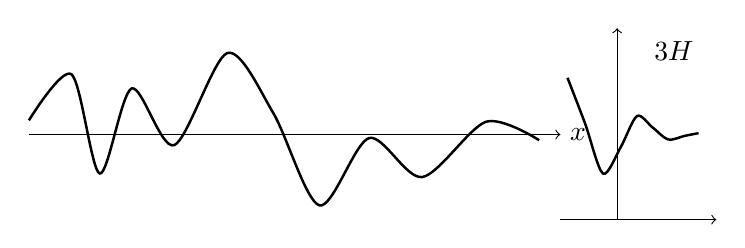
\begin{tikzpicture}[scale=0.9]
\draw[->] (0,0) -- (7.5,0) node[right] {$x$};
\draw[line width=0.9pt] plot[smooth] coordinates {(0.0,0.2) (0.6,0.85) (1.0,-0.55) (1.45,0.65) (2.05,-0.15) (2.8,1.15) (3.45,0.3) (4.1,-1.0) (4.8,-0.05) (5.55,-0.6) (6.45,0.18) (7.2,-0.08)};
\draw[->] (8.3,-1.2) -- (8.3,1.5);
\draw[->] (7.5,-1.2) -- (9.7,-1.2);
\draw[line width=0.9pt] plot[smooth] coordinates {(7.6,0.8) (7.85,0.15) (8.1,-0.55) (8.35,-0.18) (8.58,0.26) (8.8,0.1) (9.02,-0.07) (9.25,-0.02) (9.45,0.02)};
\node at (9.1,1.18) {$3H$};
\end{tikzpicture}
\caption{A cleaned qualitative picture: a frozen field profile built from many wavelengths, together with a damped-oscillation inset.}
\end{figure}

This is not yet enough. If there were only a fixed initial population of waves, then expansion would eventually stretch them all to enormous size and the field would become featureless. The lecture therefore adds a second ingredient: vacuum fluctuations are always present. New short-wavelength modes are continually supplied by zero-point motion. They begin with short wavelength, oscillate, stretch, cross the horizon, and freeze. Then the next short-wavelength modes do the same. The field that remains after many such events is a superposition of frozen modes of many wavelengths and orientations. That is the lecture's qualitative explanation of a scale-spanning, nearly scale-invariant pattern.

\section{Falling Off The Cliff: From Frozen Field Noise To Density Perturbations}

Up to this point we have explained how the inflaton field acquires a frozen, spatially varying pattern. But the lecture insists on a further point: the energy stored in those tiny quantum waves is not itself enough to account for the observed density contrasts. Something else must amplify their effect. That amplification occurs when the field reaches the edge of the plateau.

First imagine no noise at all. Then \(\phi\) has the same value everywhere in space. The field drifts slowly along the flat plateau, reaches the cliff, and the whole universe falls off together. The potential energy is converted into particles, radiation, and heat. Exponential expansion ends. Ordinary matter and radiation then dilute as the universe expands.

\begin{figure}[htbp]
\centering

\includegraphics[width=0.86\textwidth]{lecture_10_figure_05.png}
\caption{The blackboard sketch in which horizontal position is \(\phi\), vertical position is space, and successive field profiles drift toward the cliff at the right edge.}
\end{figure}

\begin{figure}[htbp]
\centering
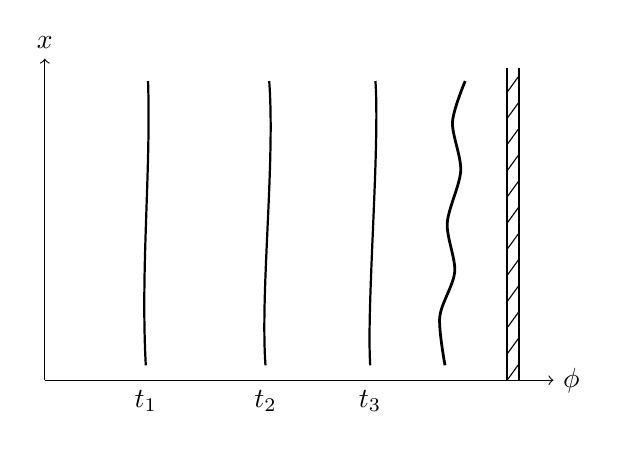
\begin{tikzpicture}[scale=0.95]
\draw[->] (0,0) -- (6.8,0) node[right] {$\phi$};
\draw[->] (0,0) -- (0,4.3) node[above] {$x$};

\draw[line width=0.8pt] (1.35,0.2) .. controls (1.28,1.5) and (1.42,2.8) .. (1.38,4.0);
\draw[line width=0.8pt] (2.95,0.2) .. controls (2.88,1.2) and (3.08,2.9) .. (3.00,4.0);
\draw[line width=0.8pt] (4.35,0.2) .. controls (4.30,1.0) and (4.48,3.1) .. (4.42,4.0);
\draw[line width=1.0pt] plot[smooth] coordinates {(5.35,0.2) (5.28,0.85) (5.48,1.45) (5.38,2.1) (5.56,2.8) (5.45,3.45) (5.62,4.0)};

\draw[line width=1.0pt] (6.18,0.0) -- (6.18,4.18);
\draw[line width=1.0pt] (6.34,0.0) -- (6.34,4.18);
\foreach \y in {0.0,0.35,0.7,1.05,1.4,1.75,2.1,2.45,2.8,3.15,3.5,3.85}{
\draw (6.18,\y) -- (6.34,\y+0.22);
}

\node[below] at (1.35,0) {$t_1$};
\node[below] at (2.95,0) {$t_2$};
\node[below] at (4.35,0) {$t_3$};
\end{tikzpicture}
\caption{A cleaned reconstruction of the lecture's space-versus-\(\phi\) picture. Each nearly vertical line is the field profile at a later time, drifting toward the cliff at the right.}
\end{figure}

Now put the noise back. The frozen modes mean that the field is not exactly the same at every point. It wanders slightly across space. The lecture gives a memorable picture: think of a line of people walking toward the cliff while trying to stay abreast. A few are slightly ahead; a few are slightly behind. The ones who are ahead go over first.

That timing difference is the amplification mechanism. A region that falls first reheats first. Its potential energy is dumped into particles and radiation, and then that energy begins to dilute. A nearby region that falls a little later reheats later, so by the time we compare the two, the later region is denser simply because it has had less time to dilute. Thus a tiny fluctuation in \(\phi\) is turned into a larger fluctuation in energy density.

The lecture does not present a formal perturbation-theory calculation here. It presents the mechanism. The result is a complicated hierarchy of overdense and underdense pockets, of many sizes nested inside one another. That is the sense in which the pattern is fractal. The net density contrast may then be summarized as
\begin{equation}
\frac{\delta\rho}{\rho}\sim 10^{-5},
\end{equation}
with the detailed amplitude depending on the shape of the potential and the speed of the roll.

One qualitative dependence is singled out explicitly. The slower the field rolls, the larger the effect. If \(\dot \phi\) is smaller, then the time interval between one region going over the cliff and another region following it is longer, and more dilution can occur in between. So a slower roll enhances the final density contrast.

At this point the bridge back to WMAP is complete. The density fluctuations created by staggered reheating later become the seeds of galaxy formation. But before galaxies form, the last-scattering surface passes through this inhomogeneous matter distribution. Photons coming from denser regions are redshifted differently from photons coming from less dense regions, and the microwave sky records exactly that shell of structure. We do not see the whole three-dimensional pattern at once. We see its imprint on the last-scattering surface.

The lecture closes with two brief cautions. First, the microwave background is not radiation from time zero; it formed only after the universe had cooled for hundreds of thousands of years after reheating. Second, large-angle anomalies in the microwave sky should be treated with restraint. On very large angular scales there is only one realization available to observe. This is the regime of cosmic variance: one can do statistics on many small-scale fluctuations, but not on the unique quadrupole of our one observable universe.

\section{Summary}

The lecture's logic is compact once one sees it in the right order. Planck units remind us that cosmology must connect low-energy physics to extremely fundamental scales. WMAP then poses the empirical problem: the universe is almost homogeneous, but not exactly, and the deviations are of order \(10^{-5}\) with approximate scale invariance. To answer that problem we need only a scalar field in an expanding universe, the zero-point motion of a harmonic oscillator, and the dynamics of damping.

Inflation turns each Fourier mode of the inflaton into a damped oscillator with a time-dependent restoring force. As expansion stretches the mode and weakens its restoring force, the mode crosses from oscillatory behavior to overdamped behavior and freezes when its wavelength reaches the Hubble scale. Those frozen fluctuations by themselves are tiny, but they modulate the time at which different regions fall off the inflaton cliff and reheat. Early-reheated regions dilute more; late-reheated regions dilute less. In that way a quantum fluctuation in \(\phi\) becomes a density fluctuation in matter, and that density fluctuation becomes the pattern later seen in the microwave background and in large-scale structure.